\documentclass[bigger]{beamer}
%\documentclass[handout]{beamer}
\setbeamertemplate{bibliography item}{}
\usepackage[utf8]{inputenc}
\usepackage[english]{babel}
\usepackage{multirow}
\usepackage{synttree}
\usepackage{booktabs}
\usepackage[backend=bibtex,natbib,style=authoryear]{biblatex}
\usetheme{Warsaw}
%\usefonttheme[onlylarge]{structuresmallcapsserif}
\newcommand{\wigegraph}[1]{\begin{figure}[h]
\centering\includegraphics[width=\textwidth]{#1}\end{figure}}
% Ez most valamiert besz.rt, ugyhogy kikommentalom:
%\AtBeginSection[]{\frame{\frametitle{Outline}\tableofcontents[current]}}

\AtBeginPart{\frame{\partpage}} 

\usepackage{tikz}
\usepackage{tikz-qtree}
\usepackage{xspace}

\bibliography{ml}

\newcommand{\defl}{\texttt{dep\_to\_4lang}\xspace}
\newcommand{\difl}{\texttt{dict\_to\_4lang}\xspace}
\newcommand{\tfl}{\texttt{text\_to\_4lang}\xspace}
\newcommand{\tefl}{\texttt{text\_to\_4lang}\xspace}
\newcommand{\fl}{\texttt{4lang}\xspace}

\newcommand{\edge}[3]{\texttt{#1}~$\xrightarrow#2$~\texttt{#3}}
\newcommand{\twoedges}[4]{\texttt{#1}~$\overset{#2}{\underset{#3}{\rightleftharpoons}}$~\texttt{#4}}
\newcommand{\bin}[3]{
    \texttt{#2}~$\xleftarrow1$~\texttt{#1}~$\xrightarrow2$~\texttt{#3}}

\newcommand{\todo}[1]{\textbf{TODO: #1}}

%\usepackage{apacite}
%\let\cite\shortcite  % to get "et al." for more than two authors
%\let\citeA\shortciteA
\begin{document}

\title{Knowledge base population using natural language inference}
\author{\'Ad\'am Kov\'acs}
\institute{Department of Automation and Applied Informatics \\
Budapest University of Technology and Economics \\
\texttt{adaam.ko@gmail.com}}

\date{AACS'18\\
06/22/2018}

%-----------------------

\begin{frame} 

\titlepage 

\end{frame} 

%-----------------------
%-----------------------

\begin{frame} 

    \frametitle{KBP \citep{HengJi:2011}} 
    \begin{itemize}
        \pause \item Goal: discover facts about entities and augment a knowledge base with these facts
        \pause \item General systems diverge from our solution
        \begin{itemize}
            \pause \item Unstructured data
            \pause \item We use inference
        \end{itemize}
        \pause \item Knowledge base: WikiData
        \pause \item Semantic graphs: 4lang
    \end{itemize}

\end{frame} 

%-----------------------


%-----------------------
{
\setbeamerfont{frametitle}{size=\small}

\begin{frame}
    \frametitle{\fl: the formalism \citep{Kornai:2010,Kornai:2015a}}
\pause Directed graphs of concepts, with 3 types of edges:
\begin{itemize}
    \pause \item 0-edges
        \begin{itemize}
            \pause \item attribution: \texttt{dog}~$\xrightarrow0$~\texttt{large}
            \pause \item \texttt{IS\_A} relation (hypernymy): \texttt{dog}~$\xrightarrow0$~\texttt{mammal}
            \pause \item unary predication: \texttt{dog}~$\xrightarrow0$~\texttt{bark}
        \end{itemize}
    \pause \item 1- and 2-edges connect binary predicates to their arguments.
\end{itemize}
\pause \begin{figure}
\centering
    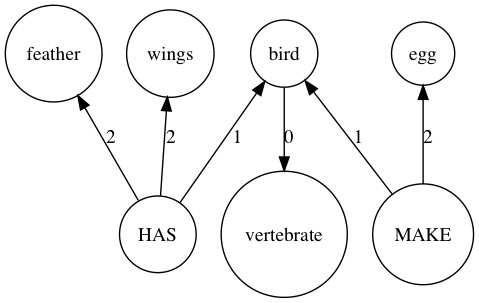
\includegraphics[scale=0.4]{pics/bird.jpg}
\end{figure}
\end{frame}
}
%-----------------------

\begin{frame}
    \frametitle{The \difl module \citep{Recski:2016d}}
    \pause \begin{figure}
    \centering
    \small
        Job is \textit{the regular paid work that you do for an employer}
        \pause \[\Downarrow\]
        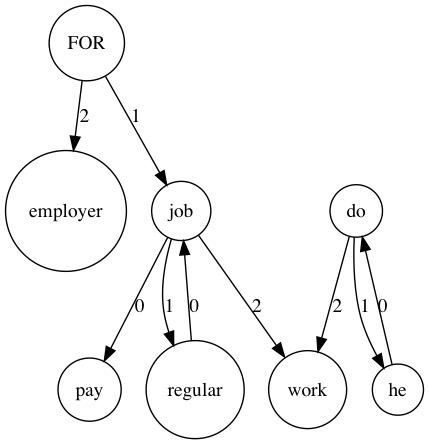
\includegraphics[scale=0.4]{pics/job.jpg}
    \label{fig:job}
    \end{figure}
    
    \end{frame}
%-----------------------
\begin{frame}
    \frametitle{\fl: WikiData}
\begin{itemize}
    \pause \item Public domain knowledge base
    \pause \item 30 million entities
    \pause \item Structured (Json dump)
    \pause \item For each entity pairs of \texttt{properties} and \texttt{values}
    \pause \item Relation triplets
        \begin{itemize}
            \pause \item author(George Orwell, 1984)
        \end{itemize}
\end{itemize}

\end{frame}
%-----------------------
\begin{frame}
    \frametitle{\fl: Method}
    \centering
    \pause author(George Orwell, 1984)
    \begin{columns}
        \begin{column}{0.4\textwidth}
            \pause 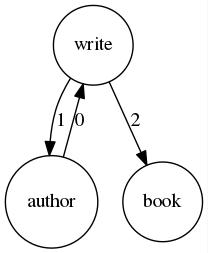
\includegraphics[scale=0.6]{pics/author.jpg}
        \end{column}
        \begin{column}{0.6\textwidth}
            \begin{itemize}
                \pause \item R(X, Y)
                \pause \item If \texttt{R}~$\xrightarrow0$~\texttt{Z} then \texttt{X}~$\xrightarrow0$~\texttt{Z}
                \begin{itemize}
                    \pause \item \texttt{Orwell}~$\xrightarrow0$~\texttt{write}
                \end{itemize}
                \pause \item If \texttt{R}~$\xrightarrow0$~\texttt{Z}~$\xrightarrow2$~\texttt{W} then \texttt{Y}~$\xrightarrow0$~\texttt{W}
                    \begin{itemize}
                        \pause \item \texttt{1984}~$\xrightarrow0$~\texttt{book}
                    \end{itemize}
            \end{itemize}
        \end{column}
    \end{columns}
\end{frame}
%-----------------------
\begin{frame}
    \frametitle{\fl: Method}
    \begin{figure}
        \centering
        \small
            author(George Orwell, 1984)
            \[\Downarrow\]
            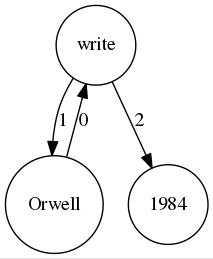
\includegraphics[scale=0.6]{pics/orwell_inf.jpg}
        \label{fig:method}
        \end{figure}
\end{frame}
%-----------------------
\begin{frame}
    \frametitle{\fl: Errors}
    \begin{itemize}
        \pause \item employer (CIA, Mike Pompeo)
            \begin{itemize}
                \pause \item is a person, company, or organization that employs people
                \pause \item \texttt{CIA}~$\xrightarrow0$~\texttt{Person}
            \end{itemize}
        \pause \item Meaningless
            \begin{itemize}
                \pause \item \texttt{flag}~$\xrightarrow0$~\texttt{piece}
            \end{itemize}
        \pause \item WikiData errors
    \end{itemize}
\end{frame}
%-----------------------

\begin{frame}
    \frametitle{\fl: Evaluation}
    \begin{figure}
        \centering
        \small
            WikiData(86.3m triplets and 893 unique predicates)
            \pause \[\Downarrow\]
            Preprocessing
            \pause \[\Downarrow\]
            Keep graphs with exactly one outgoing 0- or 2-edge or no incoming edges
            \pause \[\Downarrow\]
            Apply our each pattern
            \pause \[\Downarrow\]
            Manual inspection
         \label{fig:eval}
        \end{figure}

\end{frame}

%-----------------------
\begin{frame}
    \frametitle{\fl: Manual inspection}
    \begin{columns}
        \begin{column}{0.4\textwidth}
            \pause 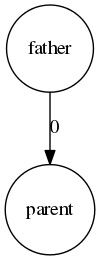
\includegraphics[scale=0.6]{pics/father.jpg}
        \end{column}
        \begin{column}{0.6\textwidth}
            \begin{figure}
                \centering
                \small
                If \texttt{X}~$\xrightarrow0$~\texttt{Father} implies \texttt{X}~$\xrightarrow0$~\texttt{Parent} 
                \pause \[\Downarrow\] Each inferred fact is correct
                \label{fig:manual}
            \end{figure}
        \end{column}
    \end{columns}
\end{frame}
%-----------------------

\begin{frame}
\frametitle{Results}
\begin{table}
    \centering
    \begin{tabular}{lrrr}
                    & 1-pattern & 2-pattern & total\\
        predicates  & 84 & 25 & 109 \\
        correct     & 55 & 17 & 72 \\
        new facts   & 8.2 million & 0.83 million & 9 million \\
        correct     & 7.6 million & 0.74 million & 8.3 million \\ 
        accuracy    & 0.92 & 0.89 & 0.92
    \end{tabular}
    \caption{Evaluation results}
    \label{table:results}
\end{table}
\end{frame}

%-----------------------

\begin{frame}
\frametitle{Conclusion}
\begin{itemize}
    \pause \item We used simple pattern-based methods for a KBP task
    \pause \item High-quality facts for augmenting a KB
    \pause \item Powerful method for enriching any natural language data
    \pause \item Full pipeline avaliable \url{https://github.com/adaamko/4lang}
    \pause \item Available Rest API and online demo \url{http://4lang.hlt.bme.hu}
\end{itemize}

\end{frame}
%-----------------------
%-----------------------
\begin{frame}
    \frametitle{Thank you!}
    \AtNextBibliography{\tiny}
    \printbibliography
\end{frame}
%-----------------------



\end{document}






